\documentclass{article}

\usepackage[paperwidth=16cm, paperheight=16cm]{geometry}

\usepackage{amsmath}

\usepackage{tikz}
\usetikzlibrary{decorations.pathreplacing}

\begin{document}

\pagestyle{empty}

\begin{center}
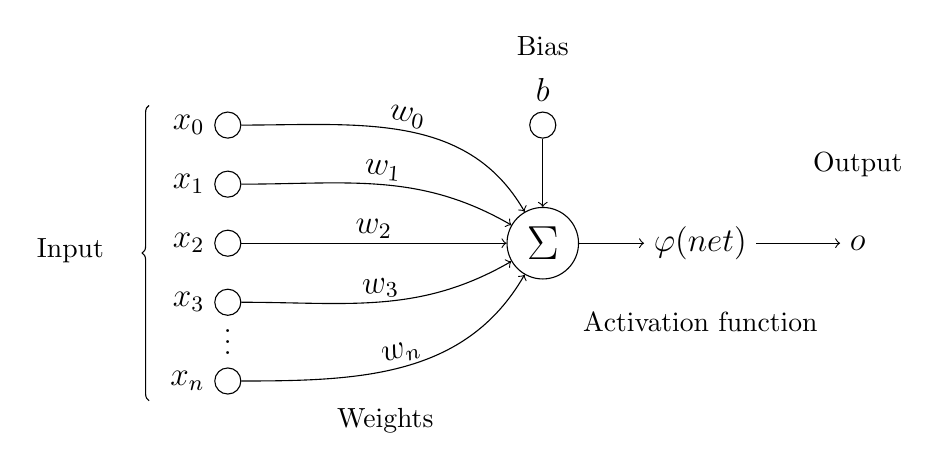
\begin{tikzpicture}
    \tikzstyle{input}=[draw, circle, minimum size=5pt]
    
    % Input
	\node[input, label=left: \large{$x_0$}] (x0) at (-2, 1.5) {};
	\node[input, label=left: \large{$x_1$}] (x1) at (-2, 0.75) {};
	\node[input, label=left: \large{$x_2$}] (x2) at (-2, 0) {};
	\node[input, label=left: \large{$x_3$}] (x3) at (-2, -0.75) {};
	\node (dots) at (-2, -1.15) {$\vdots$};
	\node[input, label=left: \large{$x_n$}] (xn) at (-2, -1.75) {};
	
	% Bias
	\node[input, label=above: \large{$b$}] (b) at (2, 1.5) {};
	
	% Neuron
	\node[draw, circle, minimum size=25pt] (n) at (2, 0) {\LARGE{$\Sigma$}};
	
	% Output
	\node (f) at (4, 0) {\large{$\varphi(net)$}};
	\node (o) at (6, 0) {\large{$o$}};

    % Connections
	\draw[->] (x0) to[out=0,in=120] node [midway, sloped, above=-2] {\large{$w_0$}} (n);
	\draw[->] (x1) to[out=0,in=150] node [midway, sloped, above=-2] {\large{$w_1$}} (n);
	\draw[->] (x2) to[out=0,in=180] node [midway, sloped, above=-2] {\large{$w_2$}} (n);
	\draw[->] (x3) to[out=0,in=210] node [midway, sloped, above=-2] {\large{$w_3$}} (n);
	\draw[->] (xn) to[out=0,in=240] node [midway, sloped, above=-2] {\large{$w_n$}} (n);
	
	\draw[->] (b) to node {} (n);
	
	\draw[->] (n) to node {} (f);
	\draw[->] (f) to node {} (o);
	
	% Brace
	\draw[decorate, decoration={brace, mirror}] (-3, 1.75) -- (-3, -2);
	
	% Labels
	\node at (-4, -0.1) {Input};
	\node at (0, -2.25) {Weights};
	\node[above of=b] {Bias};
	\node[below of=f] {Activation function};
	\node[above of=o] {Output};
\end{tikzpicture}
\end{center}

\vspace{1cm}

\begin{equation*}
    net_j=\sum_{i=0}^n x_i \cdot w_{ij} + b_j
\end{equation*}\\

\begin{equation*}
    o_j=\varphi(net_j)
\end{equation*}

\end{document}